\documentclass{report}
\usepackage[utf8]{inputenc}
\usepackage[top=2.5cm, left=2.3cm, right=2.7cm, bottom=3.0cm]{geometry}
\usepackage{accents}
%\usepackage{amsmath}
\usepackage{float}
\usepackage{hyperref}
\usepackage{pdfpages}
\usepackage{sectsty}
\usepackage{titlesec}
\usepackage{listings}
\usepackage{graphicx}
\graphicspath{ {./images/} }

\titleformat{\chapter}{\normalfont\huge}{\thechapter.}{20pt}{\huge\it}
\newcommand{\ubar}[1]{\underaccent{\bar}{#1}}
\newcommand{\e}[1]{\cdot10^{#1}}


\title{\huge Report HW4 \\ \Huge System Programming}
\author{\huge Baran Hasan Bozduman\\ \huge 171044036}
\date{\today}
\begin{document}
\maketitle
{\huge \textbf{Problem Definition} \\}

{\large While Reading a file with a thread, Doing some operations with other multiple threads, Cheating Student problem details in the homework pdf.\\}\\\\\\\\\\\\\\\\\\

{\huge \textbf{Design Decision} \\ \large Since the thread mutexes are not allowed I used semaphores. And we have reader writer problem here. Such as adding elements to queue or deleting elements from queue when we do these operations we should protect the operations in case of deadlocks. In my main thread firstly I read all students form file and create the related threads until these operations are done main wait for it when it reaches end of the file for student path I post the semaphore and we can start by reading the homework from homework file for after that it starts to give jobs to threads\\
    Beginning of the infinite loop first I check the available student number if there is not available student it waits until one of them available then it checks the number of homework and if there is no homework it waits to get one then it continues and takes beginning of the queue and delete that from queue then according to homework it choose a student from student array and takes its index then again in a protected area i do my operations make student busy and increase the quantity students money number of homework and update the cheater student money and then i post the semaphore of the chosen student so other threads wait until i post their semaphores, and homework money checks are they enough or all homework has done then it waits semaphore to cureent student post the information what homework he is doing\\
    In the student-for-hired thread i send the students as argument so i keep hw information within the student, it waits post operation from main for the realted student then it prints the "...is solving  homework .. for .. H has..." after that it post the semaphore so the statement has been printed and main can give a homework to next student then for that thread sleeps and when the sleeping operation done it makes its busy 0 so that student can get new homework and also post the total available students.\\
    You can see the outputs below
}



{\large  \\ For all homework done, for insufficient money, for termination signal, for valgrind leak check }
\newline
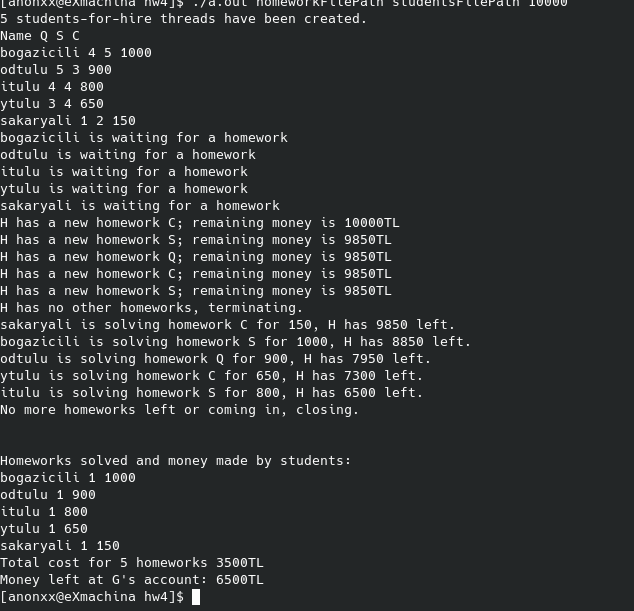
\includegraphics[width=\textwidth,height=\textheight,keepaspectratio]{images/done.png} \\
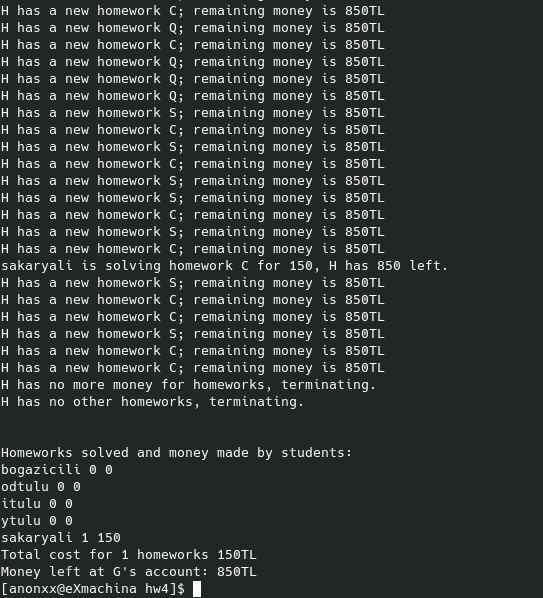
\includegraphics[width=\textwidth,height=\textheight,keepaspectratio]{images/nomoney.png}\\
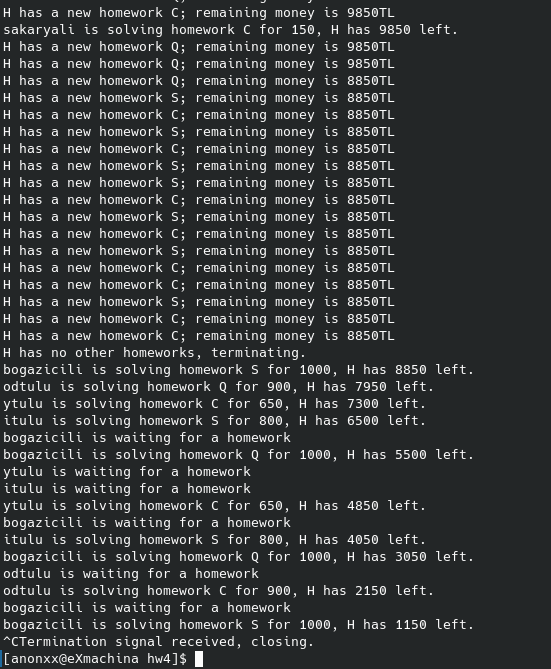
\includegraphics[width=\textwidth,height=\textheight,keepaspectratio]{images/termination.png}\\
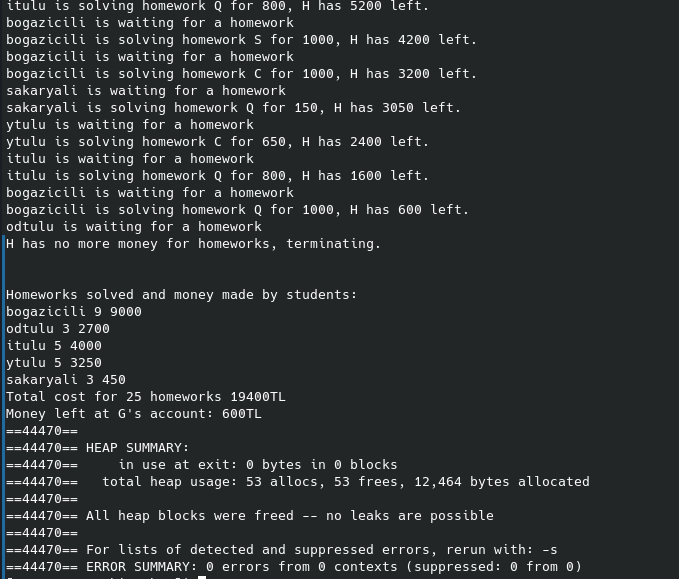
\includegraphics[width=\textwidth,height=\textheight,keepaspectratio]{images/valgrind.png}\\\\\\\\\\\\\\\\\\\\\\\\\\\\\\\\\\\\\\

{\huge \textbf{The Requirements I have achieved} \\}
{\large It provides all requirements }
 {\large I tried the rules below and they worked properly on my computer}
 
\begin{enumerate}
    \item {\large No compilation error }
    \item {\large No compilation warning}
    \item {\large \check{Makefile} }
    \item {\large \check{Report in Latex format}}
    \item {\large Printed usage information in case of missing or invalid argument}
    \item {\large Program did not crashed}
    \item {\large No memory leaks}
    \item {\large No zombie process}
    \item {\large No deadlock}
    \item {\large No poor synchronization}
    \item {\large Submitted on time}
    \item {\large Informed user in case of system errors}
    
\end{enumerate}

{\huge \textbf{The Requirements I have failed} \\}

{\large \\None}


\end{document}
